\chapter[Especificação do jogo]{Especificação do jogo}

Neste capítulo, apresentamos os conceitos gerais do jogo produzido, desde o objetivo, narrativa, regras, mecânicas e funcionalidades. A especificação do jogo é um documento essencial para definir de maneira clara e detalhada todos os aspectos que compõem a experiência do jogador, servindo como guia tanto para a equipe de desenvolvimento quanto para possíveis ajustes e melhorias no decorrer do projeto. A partir desta especificação, é possível alinhar as expectativas e assegurar que o produto final atenda aos requisitos propostos, oferecendo uma base sólida para a implementação e testes do jogo.

\section{Narrativa}

O jogo tem várias inspirações, sendo a principal delas a série “Tron – Uma Odisseia Eletrônica”. Ele utiliza a mecânica dos \textit{light-cycles}, que são rastros deixados pelos jogadores no filme. \textit{Light-cycle} é um sub-jogo da série no qual o objetivo é forçar os jogadores a colidirem com a parede ou com os rastros de luz deixados pelos demais, muito similar ao clássico jogo \textit{Snake}, também conhecido como jogo da cobrinha, mas com elementos de \textit{battle royale}.

Outra inspiração relevante é o jogo de navegador “Curve Fever”, cuja proposta é semelhante à adotada neste projeto. A ideia é criar uma versão renovada do jogo para guiar o aprendizado.

\begin{figure}[htbp]
    \centering
    \caption{Jogo Achtung Die Kurve}
    \label{fig:achtung-kurve}
    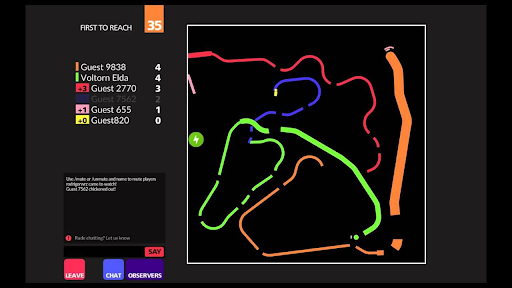
\includegraphics[width=0.7\textwidth]{figuras/kuver-fever.png}
    \legend{Fonte: https://www.youtube.com/watch?v=FHyALtYMfPY}
\end{figure}

A narrativa do jogo é relativamente simples. Até 6 jogadores podem ingressar numa sala virtual, onde cada um controla um dos 6 animais disponíveis. Cada animal é representado por uma cor específica: porco (rosa), dragão (vermelho), serpente (verde), baleia (azul), lobo (branco) e águia (amarelo).

Os jogadores competem em várias rodadas e acumulam pontos de acordo com sua colocação. O número de pontos necessários para o fim da partida é definido pela equação:

\begin{center}
    \textbf{Pontuação para vitória = número de jogadores $\times$ 5}
\end{center}

O número mínimo de jogadores para iniciar uma partida é 2. A pontuação obtida em cada rodada segue a regra:

\begin{center}
    \textbf{Pontos da rodada = número de jogadores $-$ colocação do jogador}
\end{center}

O primeiro jogador a atingir a pontuação definida é coroado como \textit{Rei dos Animais}.

\section{Objetivo do Jogo}

O objetivo do jogo é sobreviver o maior tempo possível dentro de um cenário limitado. Por se tratar de um jogo competitivo \textit{PvP}, o último jogador vivo será o vitorioso na rodada.

Para alcançar esse objetivo, os jogadores podem adotar estratégias variadas, utilizar poderes especiais que tornam a partida mais caótica, além de exigir habilidade motora para controlar seu personagem com precisão.

\section{Estrutura da Fase}

A estrutura da fase é simples: uma caixa com tamanho adaptável ao número de jogadores, fundo cinza-escuro e bordas cinza-claro. Ao lado da arena, há um placar exibindo a colocação dos jogadores.

Ao final de cada rodada, a área de jogo é limpa e os jogadores são reposicionados em suas posições iniciais.

\section{Poderes e Habilidades}

O jogo oferece uma habilidade padrão e diversos poderes especiais que surgem aleatoriamente durante a partida.

A habilidade padrão consiste em deixar um rastro letal por onde o personagem se move, capaz de eliminar qualquer jogador (inclusive o próprio). O rastro pode ocasionalmente conter brechas que permitem a passagem.

Os poderes especiais aparecem aleatoriamente no mapa. Ao serem coletados, são ativados imediatamente e têm duração de 7 segundos. Eles podem ajudar ou prejudicar o jogador que os coletou ou afetar os demais.

\begin{itemize}
    \item +Velocidade
    \item -Velocidade
    \item +Velocidade para os outros
    \item -Velocidade para os outros
    \item Inverter controles para os outros
    \item Andar em 90º
    \item Tornar bordas atravessáveis
    \item Limpar mapa
    \item Voar
    \item +Tamanho
    \item -Tamanho
\end{itemize}
\textbf{Poderes verdes:} aplicam-se somente ao jogador que os coletou.\\
\textbf{Poderes vermelhos:} afetam todos os outros jogadores.\\
\textbf{Poderes azuis:} afetam todos os jogadores.

Para uma descrição visual dos poderes, consulte o \textbf{Apêndice 2}.

\section{Mecânicas e Jogabilidade}

A mecânica do jogo: o jogador pode mover-se para a esquerda ou para a direita. No entanto, a movimentação dos personagens é limitada a curvas com raio pré-determinado. A velocidade do jogador influencia diretamente o tamanho da curva: quanto maior a velocidade, maior será o raio da curva.

\section{Gamificação e Análise Crítica}

A escolha desse tipo de jogo envolveu diversos fatores, como a facilidade de criação de \textit{assets} (arte do jogo) e desenvolvimento curto devido ao prazo de tempo. Reforçando a ideia deste projeto ser utilizá-lo como estudo de caso, visando gerar resultados relevantes para a pesquisa.

Apesar da mecânica simplificada, o jogo conta com diversas funcionalidades, como poderes especiais e regras que o tornam dinâmico e interessante.

Para a avaliação do engajamento, utilizou-se o \textit{framework} Octalysis, desenvolvido por Yu-kai Chou, originalmente voltado para gamificação de atividades e comportamentos. Embora seu uso mais comum esteja relacionado a sistemas gamificados em contextos educacionais e corporativos, o Octalysis também é aplicável ao \textit{game design} digital, pois fornece uma compreensão aprofundada das motivações que mantêm os jogadores envolvidos. Ele já foi utilizado em pesquisas de experiência do usuário (UX) em jogos digitais para identificar pontos de engajamento e orientar melhorias no design, como no caso documentado de \textit{Candy Crush} \cite{gamedeveloper2021octalysis}.

O framework é composto por oito \textit{cores} (impulsionadores motivacionais). Cada um representa um aspecto-chave da motivação humana que pode ser explorado em um jogo. Nesta análise, selecionamos os principais \textit{cores} presentes no protótipo e os avaliamos com base na percepção de três testadores, incluindo o autor, em uma escala de 1 a 5, onde 1 indica presença pouco explorada e 5 indica presença fortemente explorada \cite{octalysis}.

O número reduzido de participantes se deveu a limitações de tempo e disponibilidade durante a etapa de testes. Ainda que a amostra pequena limite a generalização dos resultados, ela foi suficiente para apontar ajustes iniciais nas mecânicas e confirmar elementos que contribuíram para o engajamento. O formulário de avaliação completo e os resultados estão disponíveis no Anexo~\ref{anexo:formulario}.

\subsection*{Principais \textit{cores} utilizados}

\textbf{Epic Meaning}
\textit{Resumo}: Este \textit{core} refere-se ao senso de propósito maior ou missão.
\textit{Uso}: 1 — Embora a narrativa tente envolver os animais na floresta, ela não é muito explorada e ficou desconexa do tema Tron. Os jogadores não ficaram interessados infelizmente e acabou sendo uma prospota que aos poucos foi perdendo prioridade.

\vspace{0.5em}
\textbf{Social Influence \& Relatedness}
\textit{Resumo}: Relacionado à interação social e senso de comunidade.
\textit{Uso}: 4 — Como o jogo é competitivo, a interação entre os jogadores é um ponto-chave. A disputa aumenta o engajamento e a imersão, estimulando o sentimento de conexão e rivalidade. Houve problemas em alocar muitas pessoas em um único teclado, mas foi uma bagunça divertida que reuniu amigos e situações engraçadas.

\vspace{0.5em}
\textbf{Unpredictability \& Curiosity}
\textit{Resumo}: Este \textit{core} envolve a curiosidade e o desejo de explorar.
\textit{Uso}: 4 — A presença de poderes aleatórios e a variabilidade no comportamento dos jogadores tornam o jogo imprevisível, mantendo o jogador curioso sobre os resultados de cada partida.

\vspace{0.5em}
\textbf{Loss \& Avoidance}
\textit{Resumo}: Refere-se ao medo de perder e à motivação para evitar consequências negativas.
\textit{Uso}: 3 — Embora o jogo seja competitivo, a perda não é tratada como uma consequência punitiva. A penalização ocorre principalmente na pontuação, com perdas menores nas rodadas, o que suaviza o impacto da derrota, mas ainda causa irritação nos jogadores.
